\documentclass[9pt,a5paper,]{book}
\usepackage{lmodern}
\usepackage{amssymb,amsmath}
\usepackage{ifxetex,ifluatex}
\usepackage{fixltx2e} % provides \textsubscript
\ifnum 0\ifxetex 1\fi\ifluatex 1\fi=0 % if pdftex
  \usepackage[T1]{fontenc}
  \usepackage[utf8]{inputenc}
\else % if luatex or xelatex
  \ifxetex
    \usepackage{mathspec}
  \else
    \usepackage{fontspec}
  \fi
  \defaultfontfeatures{Ligatures=TeX,Scale=MatchLowercase}
\fi
% use upquote if available, for straight quotes in verbatim environments
\IfFileExists{upquote.sty}{\usepackage{upquote}}{}
% use microtype if available
\IfFileExists{microtype.sty}{%
\usepackage{microtype}
\UseMicrotypeSet[protrusion]{basicmath} % disable protrusion for tt fonts
}{}
\usepackage[left=2cm,right=1.2cm,top=1.5cm,bottom=1.5cm]{geometry}
\usepackage{hyperref}
\hypersetup{unicode=true,
            pdftitle={Regression Models for Count Data},
            pdfauthor={Wagner Hugo Bonat; Walmes Marques Zeviani; Eduardo Elias Ribeiro Jr},
            pdfborder={0 0 0},
            breaklinks=true}
\urlstyle{same}  % don't use monospace font for urls
\usepackage{natbib}
\bibliographystyle{apalike}
\usepackage{color}
\usepackage{fancyvrb}
\newcommand{\VerbBar}{|}
\newcommand{\VERB}{\Verb[commandchars=\\\{\}]}
\DefineVerbatimEnvironment{Highlighting}{Verbatim}{commandchars=\\\{\}}
% Add ',fontsize=\small' for more characters per line
\newenvironment{Shaded}{}{}
\newcommand{\KeywordTok}[1]{\textbf{{#1}}}
\newcommand{\DataTypeTok}[1]{\underline{{#1}}}
\newcommand{\DecValTok}[1]{{#1}}
\newcommand{\BaseNTok}[1]{{#1}}
\newcommand{\FloatTok}[1]{{#1}}
\newcommand{\ConstantTok}[1]{{#1}}
\newcommand{\CharTok}[1]{{#1}}
\newcommand{\SpecialCharTok}[1]{{#1}}
\newcommand{\StringTok}[1]{{#1}}
\newcommand{\VerbatimStringTok}[1]{{#1}}
\newcommand{\SpecialStringTok}[1]{{#1}}
\newcommand{\ImportTok}[1]{{#1}}
\newcommand{\CommentTok}[1]{\textit{{#1}}}
\newcommand{\DocumentationTok}[1]{\textit{{#1}}}
\newcommand{\AnnotationTok}[1]{\textit{{#1}}}
\newcommand{\CommentVarTok}[1]{\textit{{#1}}}
\newcommand{\OtherTok}[1]{{#1}}
\newcommand{\FunctionTok}[1]{{#1}}
\newcommand{\VariableTok}[1]{{#1}}
\newcommand{\ControlFlowTok}[1]{\textbf{{#1}}}
\newcommand{\OperatorTok}[1]{{#1}}
\newcommand{\BuiltInTok}[1]{{#1}}
\newcommand{\ExtensionTok}[1]{{#1}}
\newcommand{\PreprocessorTok}[1]{\textbf{{#1}}}
\newcommand{\AttributeTok}[1]{{#1}}
\newcommand{\RegionMarkerTok}[1]{{#1}}
\newcommand{\InformationTok}[1]{\textit{{#1}}}
\newcommand{\WarningTok}[1]{\textit{{#1}}}
\newcommand{\AlertTok}[1]{\textbf{{#1}}}
\newcommand{\ErrorTok}[1]{\textbf{{#1}}}
\newcommand{\NormalTok}[1]{{#1}}
\usepackage{longtable,booktabs}
\usepackage{graphicx,grffile}
\makeatletter
\def\maxwidth{\ifdim\Gin@nat@width>\linewidth\linewidth\else\Gin@nat@width\fi}
\def\maxheight{\ifdim\Gin@nat@height>\textheight\textheight\else\Gin@nat@height\fi}
\makeatother
% Scale images if necessary, so that they will not overflow the page
% margins by default, and it is still possible to overwrite the defaults
% using explicit options in \includegraphics[width, height, ...]{}
\setkeys{Gin}{width=\maxwidth,height=\maxheight,keepaspectratio}
\IfFileExists{parskip.sty}{%
\usepackage{parskip}
}{% else
\setlength{\parindent}{0pt}
\setlength{\parskip}{6pt plus 2pt minus 1pt}
}
\setlength{\emergencystretch}{3em}  % prevent overfull lines
\providecommand{\tightlist}{%
  \setlength{\itemsep}{0pt}\setlength{\parskip}{0pt}}
\setcounter{secnumdepth}{5}
% Redefines (sub)paragraphs to behave more like sections
\ifx\paragraph\undefined\else
\let\oldparagraph\paragraph
\renewcommand{\paragraph}[1]{\oldparagraph{#1}\mbox{}}
\fi
\ifx\subparagraph\undefined\else
\let\oldsubparagraph\subparagraph
\renewcommand{\subparagraph}[1]{\oldsubparagraph{#1}\mbox{}}
\fi

%%% Use protect on footnotes to avoid problems with footnotes in titles
\let\rmarkdownfootnote\footnote%
\def\footnote{\protect\rmarkdownfootnote}

%%% Change title format to be more compact
\usepackage{titling}

% Create subtitle command for use in maketitle
\newcommand{\subtitle}[1]{
  \posttitle{
    \begin{center}\large#1\end{center}
    }
}

\setlength{\droptitle}{-2em}
  \title{Regression Models for Count Data}
  \pretitle{\vspace{\droptitle}\centering\huge}
  \posttitle{\par}
  \author{Wagner Hugo Bonat \\ Walmes Marques Zeviani \\ Eduardo Elias Ribeiro Jr}
  \preauthor{\centering\large\emph}
  \postauthor{\par}
  \date{}
  \predate{}\postdate{}

% Mathematics environments
\usepackage{amssymb}
\usepackage{amsmath}
\usepackage{amstext}

% Customize itemize's enviroments
\usepackage{enumitem}

% Fonts
\usepackage{mathpazo}
\usepackage{eulervm}
\usepackage[scaled=0.85]{beramono}
\urlstyle{tt}

% Compact toc
\usepackage{tocloft}

% Footers and headers styles
\usepackage{fancyhdr}
\pagestyle{fancy}
\fancyhf{}
\fancyhead[LE,RO]{\thepage}
\fancyhead[RE]{\scriptsize\leftmark}
\fancyhead[LO]{\scriptsize\rightmark}

% Modify color in Rcodes/chunks (works well only monochrome highlight)
\usepackage{xcolor}
\definecolor{inputcolor}{RGB}{25,25,112}
\usepackage{framed}
\usepackage{fancyvrb}
\DefineVerbatimEnvironment{Highlighting}{Verbatim}{commandchars=\\\{\},
                                                   fontsize=\small}
\definecolor{shadecolor}{RGB}{248,248,248}
\renewenvironment{Shaded}{\color{inputcolor}}{}
\renewcommand{\DataTypeTok}[1]{{#1}}

% Modify style of verbatim (chunks outputs)
\definecolor{outputcolor}{RGB}{139,0,0}
\makeatletter
\def\verbatim@font{\ttfamily \small \color{outputcolor}}%
\makeatother

\begin{document}
\maketitle

\thispagestyle{empty}
\cleardoublepage
\thispagestyle{empty}

\topskip0pt

\begin{flushleft}
  \Large \bf
  Regression Models for Count Data
\end{flushleft}
\vspace*{1.5em}

\begin{flushleft}
Wagner Hugo Bonat\\
\url{www.leg.ufpr.br/~wagner}

Walmes Marques Zeviani\\
\url{www.leg.ufpr.br/~walmes}

Eduardo Elias Ribeiro Jr\\
\url{www.leg.ufpr.br/~eduardojr}
\end{flushleft}
\vspace*{2em}

Laboratório de Estatística e Geoinformação (LEG)\\
\url{http://www.leg.ufpr.br}\\
Departamento de Estatística\\
Universidade Federal do Paraná (UFPR)

Supplementary content: \url{http://www.leg.ufpr.br/rmcd}\\
Contact: \url{rmcd@leg.ufpr.br}
\vspace*{\fill}

\begin{center}
XV EMR - Escola de Modelos de Regressão\\
Goiânia - Goiás, Brasil\\
March 26 to 29, 2017
\end{center}

\clearpage
\thispagestyle{empty}
\pagebreak

\setcounter{page}{1}

{
\setcounter{tocdepth}{1}
\tableofcontents
}
\chapter*{Preface}\label{preface}
\addcontentsline{toc}{chapter}{Preface}

The analysis of normal and non-normal data are mostly based on the class
of generalized linear models \citep{nelder1972}. The class offers a very
attractive statistical modelling framework which includes the Gaussian,
logistic and Poisson regression models for the analysis of continuous,
binomial and count data, respectively. The theoretical background for
the GLM is based on the exponential dispersion models
\citep{jorgensen1987, jorgensen1997} as a generalization of the
exponential family of distributions. Furthermore, the whole class of
models can be fitted by a simple Newton score algorithm relying only on
second-moment assumptions for estimation and inference. Despite of the
flexibility of the GLM class, the Poisson distribution is the only
choice for analysis of count data. For this reason, in practice there is
probably an over-emphasis on the use of the Poisson distribution. A well
known limitation of the Poisson distribution is the mean and variance
relationship, referred to as equidispersion. In practice, however, count
data can present other features, namely underdispersion and
overdispersion that is often related to zero-inflation, heavy tail or
absence of important explanatory variables. These features can make the
Poisson distribution unsuitable for the analysis of count data. The main
goal of this course is to present a wider range of statistical models to
deal with count data. In particular, we focus on parametric and
second-moments specified models. We shall present the model
specification along with strategies for model fitting and the associated
R code. Furthermore, a book-course and supplementary material as R
\citep{rcore2016} code and data sets will be made available for the
students. We intend to keep the course in a level suitable for bachelor
students who already attended a course on generalized linear models.
However, since the course also covers updated topics, it can be of
interest of postgraduate students and researches in general. In what
follows, we describe the course structure as well as the main
bibliography references on which the course is based. The subject
covered and the Expected learning outcome.

\chapter{Introduction}\label{introduction}

Figure \ref{fig:process-ilustration} illustrates the generator process
for under, over and equidispered counts in two dimensions context. The
grid lines in this figure indicate fixed regions for which events are
counted and the counts within each interval are displayed. For the
equidispersed case the distribution of events is random. In
overdispersed case, the events are clustered. This behaviour can be
explained by a contamination process (e.g.~count contagious disease).
The underdispersed case, in contrast of overdispersion, shows the events
distribution is nearly regular and the counts have smaller variances.
The natural process that explains underdispersion is repulsion, exactly
the opposite of overdispersion, that means, an event occurence inhibits
others near (e.g.~count territorialistas animals).

\begin{figure}[h]

{\centering 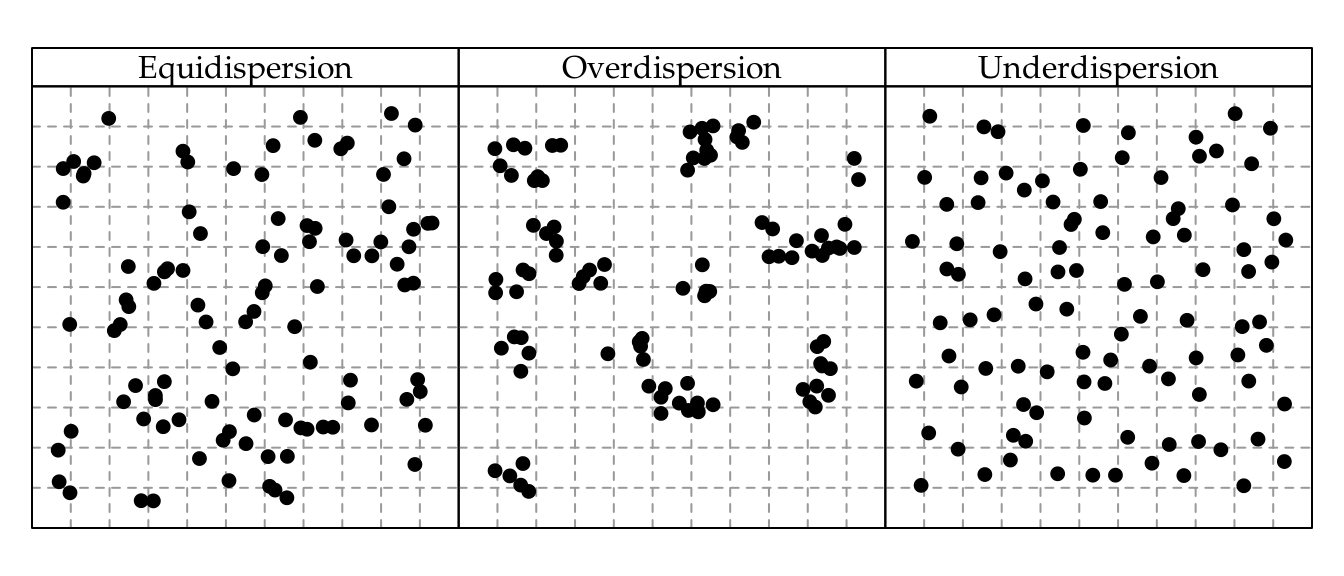
\includegraphics{rmcdbook_files/figure-latex/process-ilustration-1} 

}

\caption{Illustration of generator process for under, over and equidispered count data.}\label{fig:process-ilustration}
\end{figure}

\chapter{Background}\label{background}

\chapter{Full Parametric Approach}\label{full-parametric-approach}

\section{Models for count data}\label{models-for-count-data}

\section{Regression models}\label{regression-models}

\section{Estimation and inference}\label{estimation-and-inference}

\section{Computational
implementation}\label{computational-implementation}

\chapter{Second Moments Based
Especification}\label{second-moments-based-especification}

\section{Mean and variance
relationship}\label{mean-and-variance-relationship}

\section{Estimation functions
approach}\label{estimation-functions-approach}

\section{Extended Poisson-Tweedie regression
models}\label{extended-poisson-tweedie-regression-models}

\section{Computational
implementation}\label{computational-implementation-1}

\chapter{Data analysis}\label{data-analysis}

\section{Ovedispersed case}\label{ovedispersed-case}

\section{Underdispersed case}\label{underdispersed-case}

\subsection{Cotton bolls greenhouse
experiment}\label{cotton-bolls-greenhouse-experiment}

The data set in this section come from a greenhouse experiment with
cotton plants (Gossypium hirsutum) obtained under a completely
randomized design with five replicates. The experiment was aimed to
assess the effects of five defoliation levels (0\%, 25\%, 50\%,75\% and
100\%) on the observed number of bolls produced by plants at five growth
stages: vegetative, flower-bud, blossom, fig and cotton boll. The
experimental unity was a vase with two plants. The number of cotton
bolls was recorded at the each culture cycle. This data was analysed by
\citet{bonat2016b}, with extended Poisson-Tweedie model and
\citet{zeviani2014} with Gamma-Count model. In this section the results
of articles are reproduced and compared jointly others alternatives for
analysis (COM-Poisson model and Generalized-Poisson model).

This code below shows how to get the data and how it is structured in R.
The data set contains 125 records and 4 variables, described below:

\begin{itemize}
\item
  \texttt{defol} A numeric factor with 5 levels that represents the
  (artifitial) levels of defoliation (percent in leaf area removed with
  scissors) applied for all leaves of the plants.
\item
  \texttt{phenol} A categorical ordered factor with 5 levels that
  represents the (phenological) growth stages of the cotton plants in
  which the levels of defoliation was applied.
\item
  \texttt{rept} Integer variable that indexes each experimenal unit in
  each treatment cell.
\item
  \texttt{bolls} The number of bolls produced (count variable) evaluated
  at harvest of cotton.
\end{itemize}

\begin{Shaded}
\begin{Highlighting}[]
\NormalTok{## Read the data via package book}
\NormalTok{cotton <-}\StringTok{ }\KeywordTok{read.table}\NormalTok{(}\StringTok{"./data/cotton.csv"}\NormalTok{, }\DataTypeTok{header =} \OtherTok{TRUE}\NormalTok{,}
                     \DataTypeTok{sep =} \StringTok{";"}\NormalTok{)  ## Remove this}
\NormalTok{## data(cotton, package = "rmcd")}

\NormalTok{## ## or read the data via url address}
\NormalTok{## url <- "http://cursos.leg.ufpr.br/rmcd/data/cotton.csv"}
\NormalTok{## cotton <- read.table(url, header = TRUE, sep = ";")}

\KeywordTok{str}\NormalTok{(cotton)}
\end{Highlighting}
\end{Shaded}

\begin{verbatim}
## 'data.frame':    125 obs. of  4 variables:
##  $ phenol: Factor w/ 5 levels "blossom","boll",..: 5 5 5 5 5 5 5 5 5 5 ...
##  $ defol : num  0 0 0 0 0 0.25 0.25 0.25 0.25 0.25 ...
##  $ rept  : int  1 2 3 4 5 1 2 3 4 5 ...
##  $ bolls : int  10 9 8 8 10 11 9 10 10 10 ...
\end{verbatim}

Figure \ref{fig:cotton} shows the number of cotton bolls recorded for
each combination of defoliation level and growth stage.

\begin{figure}[h]

{\centering 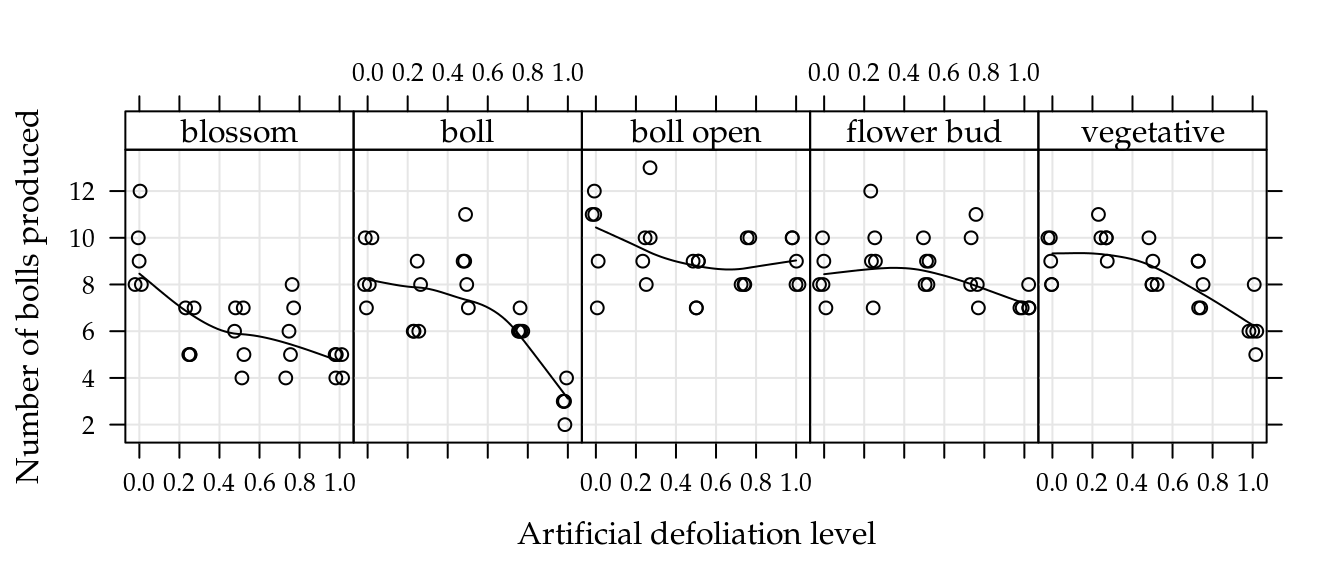
\includegraphics{rmcdbook_files/figure-latex/cotton-1} 

}

\caption{Number of bolls produced for each artificial defoliation level and each growth stage.}\label{fig:cotton}
\end{figure}

\section{Equidispersed case}\label{equidispersed-case}

\section{Zero-Inflated case}\label{zero-inflated-case}

\chapter{Discussion}\label{discussion}

\bibliography{rmcd.bib}


\end{document}
